\documentclass[11pt, addpoints]{exam}

\usepackage{amsmath, amssymb, amsthm, euler}
\usepackage{xcolor}
\usepackage{graphicx}
\usepackage{graphics}
\usepackage{tikz}
\usepackage{tikz-qtree}
\usetikzlibrary{graphs}
\tikzset{every tree node/.style={minimum width=2em,draw,circle},
    blank/.style={draw=none},
    edge from parent/.style=
    {draw,edge from parent path={(\tikzparentnode) -- (\tikzchildnode)}},
    level distance=1.2cm}
\usepackage{listings}   
\usepackage{caption}
\usepackage{algorithm}
\usepackage{algorithmicx}
\usepackage{algpseudocode}
\usepackage{underscore}
% \usepackage[top=2cm, bottom=2cm, left=2cm, right=2cm]{geometry}  
\makeatletter
\newcommand\dlmu[2][2.5cm]{\hskip1pt\underline{\hb@xt@ #1{\hss#2\hss}}\hskip3pt}
\makeatother

% For inserting code snippets.
\usepackage{listings}
\lstset{
    columns = fixed,
    basewidth = {0.5em},
    breaklines = true,
    backgroundcolor = \color{white},
    keywordstyle = \color[RGB]{40, 40, 255},
    numberstyle = \footnotesize\color{darkgray},
    commentstyle = \ttfamily\color{violet},
    basicstyle = \ttfamily,
    stringstyle = \ttfamily\color[RGB]{128, 0, 0},
    showstringspaces = false,
    language = {[11]C++},
    escapechar = \@
}
\lstnewenvironment{cpp}[1][]{\lstset{language = {[11]C++}, #1}}{}

\usepackage{tikz}

% headers, footers, titles
\newcommand{\CourseName}{CS101 Algorithms and Data Structures}
\newcommand{\HomeworkNO}{Homework 6}
\newcommand{\DueDate}{Due date: 23:59, October 30th, 2022}

\pagestyle{headandfoot}
\runningheadrule
\runningheader{\CourseName}{\HomeworkNO}{\DueDate}
\runningfooter{}{\thepage}{}

\title{
	\CourseName\\
	Fall 2022\\
	\HomeworkNO
}
\author{}
\date{\DueDate}

% formats of questions, choices, points, etc.
\qformat{\bf\thequestion. (\totalpoints\ points) \thequestiontitle\hfill}
\pointname{'}
\CorrectChoiceEmphasis{\bf\color{blue}}
\SolutionEmphasis{\color{blue}}

% We frequently use this font.
\newcommand{\ttt}{\texttt}

\begin{document}

\maketitle

\begin{enumerate}
	\item Please write your solutions in English.
	\item Submit your solutions to gradescope.com.
	\item Set your FULL name to your Chinese name and your STUDENT ID correctly in Account Settings.
	\item If you want to submit a handwritten version, scan it clearly. \ttt{CamScanner} is recommended.
	\item When submitting, match your solutions to the problems correctly.
	\item No late submission will be accepted.
	\item Violations to any of the above may result in zero points.
\end{enumerate}

\begin{questions}

\titledquestion{Multiple Choices}

Each question has \textbf{one or more} correct answer(s). Select all the correct answer(s). For each question, you will get 0 points if you select one or more wrong answers, but you will get 1 point if you select a non-empty subset of the correct answers.

Write your answers in the following table.

%%%%%%%%%%%%%%%%%%%%%%%%%%%%%%%%%%%%%%%%%%%%%%%%%%%%%%%%%%%%%%%%%%%%%%%%%%%
% Note: The `LaTeX' way to answer a multiple-choices question is to replace `\choice'
% with `\CorrectChoice', as what you did in the previous questions. However, there are 
% still many students who would like to handwrite their homework. To make TA's work 
% easier, you have to fill your selected choices in the table below, no matter whether 
% you use LaTeX or not.
%%%%%%%%%%%%%%%%%%%%%%%%%%%%%%%%%%%%%%%%%%%%%%%%%%%%%%%%%%%%%%%%%%%%%%%%%%%

\begin{table}[htbp]
	\centering
	\begin{tabular}{|p{2cm}|p{2cm}|p{2cm}|p{6cm}|}
		\hline
		(a) & (b) & (c) \\
		\hline
		%%%%%%%%%%%%%%%%%%%%%%%%%%%%%%%%%%%%%%%%%%%%%%%%%%%%%%%%%%
		% YOUR ANSWER HERE.
		  BD  &  AC   &  C   \\
		%%%%%%%%%%%%%%%%%%%%%%%%%%%%%%%%%%%%%%%%%%%%%%%%%%%%%%%%%%
		\hline
	\end{tabular}
\end{table}

\begin{parts}
	\part[2] A problem in $\NP$ is $\NPC$ if:
	\begin{choices}
		\choice It can be reduced to another $\NPC$ problem in polynomial time.
		\CorrectChoice There exists a $\NPC$ problem which can be reduced to it in polynomial time.
		\choice It can be reduced to any other $\NP$ problem in polynomial time.
		\CorrectChoice Any other $\NP$ problem can be reduced to it in polynomial time.
	\end{choices}


	\part[2] Assuming that $\P\neq\NP$, which of the following problems are in $\NPC$?
	You may search the Internet for more information if you are unfamiliar with the problems.
	\begin{choices}
		\CorrectChoice \texttt{LONG-PATH}: $(G,s,t,k)$ Given an undirected graph $G$,
		determine whether there exists a simple path from \(s\) to \(t\) whose length is greater or equal to $k$.
		\choice \texttt{HALTING}: $(P,I)$ Given a compilable C++ program $P$ and the input $I$ for $P$,
		determine if $P$ runs infinitely on $I$.
		\CorrectChoice \texttt{4-SAT}: $\phi$ Given a CNF (conjunction normal form)
		where each clause is the disjunction of exactly 4 literals,
		determine whether $\phi$ is satisfiable.
		\choice \texttt{PRIME}: $n$ Given a positive integer $n$, determine whether it is a prime number.
	\end{choices}

	\part[2] For two decision problems $A$ and $B$, suppose that $A\leq_p B$.
	Which of the following statements are true?
	(Hint: there exists complexity classes that are strictly bigger than $\NP$)
	\begin{choices}
		\choice $A\in \P \implies B\in \P$
		\choice $A\in \NPC\implies B\not\in \NPC$.
		\CorrectChoice $B\in \P\implies A\in \P$.
		\choice $B\in \NPC\implies A\in \NPC$.
	\end{choices}

\end{parts}


\newpage

\titledquestion{BST and AVL tree}

\begin{parts}
    \part[3] Draw a valid BST of minimum height containing the keys 1, 2, 4, 6, 7, 9, 10.\\\\\\\\
    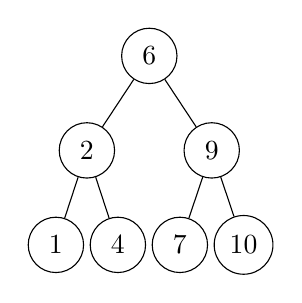
\begin{tikzpicture}
    \Tree
    [.6
        \edge[]; [.2
                \edge[]; [.1 ]
                \edge[]; [.4 ]
            ]
        \edge[]; [.9
                \edge[]; [.7 ]
                \edge[]; [.10 ]
            ]
    ]
    \end{tikzpicture}
    \vspace{1cm}
    
    \part[4] Given an empty AVL tree, insert the sequence of integers $15, 20, 23, 10, 13, 7, 30, 25$ from left to right into the AVL tree. Draw the final AVL tree.\\\\\\\\
    
    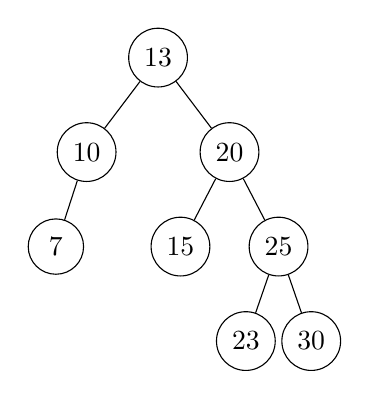
\begin{tikzpicture}
    \Tree
    [.13
        \edge[]; [.10
                \edge[]; [.7 ]
                \edge[blank]; \node[blank]{};
            ]
        \edge[]; [.20
                \edge[]; [.15 ]
                \edge[]; [.25
                    \edge[]; [.23 ]
                    \edge[]; [.30 ]
                ]
            ]
    ]
    \end{tikzpicture}
    \vspace{1cm}
   
    \part[2]For the final AVL tree in the question (b), delete $7$. Draw the AVL tree after deletion.
    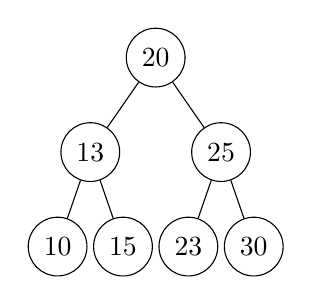
\begin{tikzpicture}
    \Tree
    [.20
        \edge[]; [.13
                \edge[]; [.10 ]
                \edge[]; [.15 ]
            ]
        \edge[]; [.25
                \edge[]; [.23 ]
                \edge[]; [.30 ]
            ]
    ]
    \end{tikzpicture}
    \vspace{1cm}
   
   \newpage
   
   \part[5]For an AVL tree, define D = the number of descendants of the left child of the root - the number of descendants of the right child of the root. Then what is the maximum of D for an AVL tree with height n? 
   
   $D_{max}=k_1\times 2^n+k_2\times B^n+k_3\times(-\frac{1}{B})^n$, please write down the value of B and $k_i$.
   
   since we want to make $D_{max}$\\
   so we can make the number of descendants of the left child of the root as big as possible,\\
   and make the number of descendants of the right child of the root as small as possible.\\
   for the left child, the max situation is that the left subtree is a perfect tree with the height of $n-1$,
   and since its height is $n-1$,so its number of nodes is $2^n-1$.\\
   and for right subtree, the min number of nodes to mention the tree as a AVL tree,\\
   so the min height of the right subtree is $n-2$, and the number is min nodes with height of $n-2$ is  
   $F(n-2)=\frac{1}{\sqrt{5}}[(\frac{\sqrt{5}+1}{2})^{n+1}-(\frac{1-\sqrt{5}}{2})^{n+1}]-1$\\
   so $D_{max}=$left\_max\_number-right\_min\_number$=2^n-1-\{\frac{1}{\sqrt{5}}[(\frac{\sqrt{5}+1}{2})^{n+1}-(\frac{1-\sqrt{5}}{2})^{n+1}]-1\}$\\
   $=2^n-\frac{1}{\sqrt{5}}(\frac{\sqrt{5}+1}{2})^{n+1}+\frac{1}{\sqrt{5}}(-\frac{1}{\frac{\sqrt{5}+1}{2}})^{n+1}$\\
   $=2^n-\frac{1+\sqrt{5}}{2\sqrt{5}}(\frac{\sqrt{5}+1}{2})^n+\frac{1-\sqrt{5}}{2\sqrt{5}}(-\frac{1}{\frac{\sqrt{5}+1}{2}})^n$\\
   $=k_1\times 2^n+k_2\times B^n+k_3\times(-\frac{1}{B})^n$\\\\
   so above all\\
   $k_1=1$\\
   $k_2=-\frac{1+\sqrt{5}}{2\sqrt{5}}$\\
   $k_3=\frac{1-\sqrt{5}}{2\sqrt{5}}$\\
   $B=\frac{\sqrt{5}+1}{2}$
   

\end{parts}

\newpage

\titledquestion{Huffman Coding}

After you compress a text file using Huffman Coding Algorithm, you accidentally spilled some ink on it and you found that one word becomes unrecognizable. Now, you need to recover that word given the following information:\\

    \textbf{Huffman-Encoded sequence of that word: } \\
    11101001011111101\\
    \textbf{Frequency table that stores the frequency of some characters: }\\
    \begin{table}[!hbtp]
    \centering
    \begin{tabular}{|l|l|l|l|l|l|l|l|l|}
    \hline
    characters & 0 & 1 & a & b & c & d & s \\ \hline
    frequency  & 2 & 3 & 3 & 4 & 1 & 4 & 2 \\ \hline
    \end{tabular}
    \end{table}\\\\
\begin{parts}	
	\part[5] Please construct the binary Huffman Coding Tree according to the given frequency table and draw the final tree below.\\
	Note: The initial priority queue is given as below. When popping nodes out of the priority queue, the nodes with the same frequency follows ``First In First Out".
		
	\begin{table}[!hbtp]
	\centering
    \begin{tabular}{|l|l|l|l|l|l|l|}
    \hline
    \begin{tabular}[c]{@{}l@{}}c\\ 1\end{tabular} & \begin{tabular}[c]{@{}l@{}}0\\ 2\end{tabular} & \begin{tabular}[c]{@{}l@{}}s\\ 2\end{tabular} & \begin{tabular}[c]{@{}l@{}}1\\ 3\end{tabular} & \begin{tabular}[c]{@{}l@{}}a\\ 3\end{tabular} & \begin{tabular}[c]{@{}l@{}}b\\ 4\end{tabular} & \begin{tabular}[c]{@{}l@{}}d\\ 4\end{tabular} \\ \hline
    \end{tabular}
    \end{table}
    
    \vspace{2cm}

    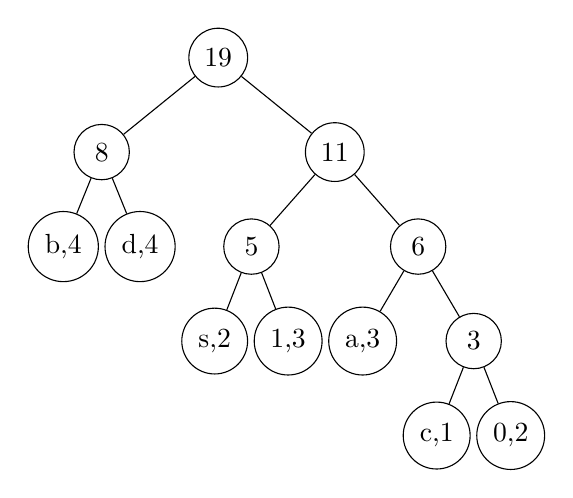
\begin{tikzpicture}
    \Tree
    [.19
        \edge[]; [.8
                    \edge[]; [.b,4 ]
                    \edge[]; [.d,4 ]
                ]
        \edge[]; [.11
                    \edge[]; [.5
                                \edge[]; [.s,2 ]
                                \edge[]; [.1,3 ]
                            ]
                    \edge[]; [.6
                                \edge[]; [.a,3 ]
                                \edge[]; [.3
                                            \edge[]; [.c,1 ]
                                            \edge[]; [.0,2 ]
                                        ]
                            ]
                ]
    ]
    \end{tikzpicture}
    \vspace{2cm}

    for the inner node: the number is the frequency of all its children,\\
    for the leaf node, the thing before $,$ is the character, the thing after $,$ is the character's frequency.\\\\
	\part[3] Now you can "decompress" the encoded sequence and recover the original word you lost. Please write the original word below.
	
    the characters and their huffman code:\\
    $b \ \ 00$\\
    $d \ \ 01$\\
    $s \ \ 100$\\
    $1 \ \ 101$\\
    $a \ \ 110$\\
    $c \ \ 1110$\\
    $0 \ \ 1111$\\\\
    
    so the original word is $cs101$
	
\end{parts}

\end{questions}

\end{document}